\chapter{TINJAUAN PUSTAKA}
\label{chap:tinjauanpustaka}

% Ubah bagian-bagian berikut dengan isi dari tinjauan pustaka

\section{Penelitian Terdahulu}
\label{sec:penelitianterdahulu}

\subsection{Kontrol Kursi Roda Menggunakan Sinyal Suara Melalui Bluetooth}

Pada tahun 2023 telah dilakukan penelitian yang berjudul "Kontrol Kursi Roda Menggunakan Sinyal Suara Melalui Bluetooth" oleh Arief Wisaksono, Rachmad Aditya Pratama, dan Hindarto hindarto dari Departemen Teknik Elektro, Fakultas Sains dan Teknologi Universitas Muhammadiyah Sidoarjo \parencite{wisaksono2023kontrol}.

Pada penelitian ini dapat disimpulkan bahwa pengujian koneksi Bluetooth dan Android dapat berjalan secara optimal. Sehingga input dari Android bisa terkirim ke rangkaian Arduino Uno. Hasil pengujian koneksi memiliki waktu delay selama 4 detik hingga 6 detik. Pengujian baterai 12 Volt memiliki deviasi sebesar 0,43 serta akurasi sebesar 96,7\%. Hal ini disebabkan karena hasil dari pengukuran lebih besar daripada tegangan yang diperlukan. Akan tetapi hal tersebut tidak mempengaruhi sistem kerja alat karena tegangan 12 Volt merupakan tegangan minimum alat.

\subsection{Rancang Bangun Kursi Roda Elektrik Dengan Sistem Kontrol \emph{Joystick} Dan \emph{Smartphone} Android}

Pada tahun 2023 telah dilakukan penelitian yang berjudul "Rancang Bangun Kursi Roda Elektrik Dengan Sistem Kontrol \emph{Joystick} dan \emph{Smartphone} Android" oleh Bayu Ahityanto Wi-caksono dari Program Studi Diploma IV Rekayasa Perancangan Mekanik, Sekolah Vokasi Universitas Diponegoro \parencite{wicaksono2023rancang}.

Pada penelitian ini didapatkan kesimpulan bahwa kursi roda konvensional yang dijadikan kursi roda elektrik berhasil dijalankan dengan kecepatan maksimal 2 km/h sesuai perencanaan. Kursi roda elektrik dapat dikontrol dengan \emph{joystick} maupun dari aplikasi yang berada di \emph{smartphone} android. Kursi roda elektrik dapat berjalan dengan beban maksimal 80 kg. Terdapat beberapa saran dari penulis seperti menambahkan sandaran kepala agar pengguna lebih nyaman di kursi roda elektrik, serta pembuatan sistem aplikasi untuk pengguna \emph{smartphone} dari Apple.

\subsection{\emph{Wheelchair Control Using Bluetooth-Based Electromyography Signals}}

Telah dilakukan penelitian yang berjudul \emph{"Wheelchair Control Using Bluetooth-Based Electromyography Signals"} oleh Yoga Eko Prasetyo dari Program Studi Teknik Elektro dan Hindarto Hindarto dari Program Studi Informatika Universitas Muhammadiyah Sidoarjo \parencite{prasetyo2023wheelchair}.

Pada penelitian ini didapatkan kesimpulan bahwa durasi tunggu dari bluetooth master dengan bluetooth slave sebesar 4 detik hingga 5 detik. Pengujian sensor elektromiografi dapat berjalan dengan normal dan menghasilkan nilai yang berbeda ketika otot berkontraksi maupun relaksasi. 

\subsection{Prototipe Kursi Roda Elektrik Dengan Kendali \emph{Joystick} dan \emph{Smartphone}}

Pada tahun 2019 telah dilakukan penelitian yang berjudul "Prototipe Kursi Roda Elektrik Dengan Kendali \emph{Joystick} dan \emph{Smartphone}" oleh Andy Sadewa Junior dan Fatchul Arifin dari Program Studi Teknik Elektronika, Fakultas Teknik Universitas Negeri Yogyakarta \parencite{junior2019prototipe}.

Pada penelitian ini didapatkan kesimpulan bahwa total \emph{error} yang dihasilkan dari pengujian tegangan motor kiri dan kanan adalah sebesar 0,144\% dan rata-rata \emph{error} yang didapatkan adalah sebesar 0,024\% pada keseluruhan pengujian yang dilakukan. Pada pengujian bluetooth didapatkan kesimpulan bahwa jangkauan pengiriman optimal dari bluetooth apabila tidak ada penghalang adalah sebesar 1 meter hingga 10 meter.

\subsection{\emph{Vision-based Head Posture Control Wheelchair System Research}}

Pada tahun 2023 telah dilakukan penelitian yang berjudul \emph{"Vision-based Head Posture Control Wheelchair System Research"} oleh Pengyu Gao dari \emph{School of Information Engineering}, \emph{Shenyang University of Chemical Technology} bersama Haitao Luo dan Yuxin Li dari \emph{Department of Space Automation Technology}, \emph{Shenyang Institute of Automation}, \emph{Chinese Academy of Sciences} \parencite{10280784}.

Pada penelitian ini didapatkan kesimpulan bahwa sistem pendeteksi pose kepada berbasis Mediapipe berhasil dilakukan menggunakan metode pemodelan matematis yang dikombinasikan dengan fungsi trigonometri untuk memperkirakan sudut wajah dan arah pose kepala. Namun masih terdapat beberapa \emph{error} pada pengenalan citra karena transmisi input citra bersifat \emph{realtime}.

\section{Teori/Konsep Dasar}

\subsection{\emph{Convolutional Neural Network} (CNN)}

\emph{Convolutional Neural Network} (CNN) telah mencapai hasil yang luar biasa selama beberapa dekade terakhir dalam berbagai bidang yang terkait dengan pengenalan pola, mulai dari pemrosesan gambar hingga pengenalan suara. Aspek paling bermanfaat dari CNN adalah mengurangi jumlah parameter dalam \emph{Artificial Neural Network}. Pencapaian ini telah membantu banyak peneliti dan pengembang dalam mengembangkan model yang lebih besar guna mengatasi tugas-tugas yang kompleks yang tidak mungkin untuk diselesaikan dengan menggunakan \emph{Artificial Neural Network} klasik. Aspek penting dari CNN adalah untuk mendapatkan fitur-fitur abstrak ketika input menyebar menuju lapisan-lapisan yang lebih dalam \parencite{8308186}.

Arsitektur pada CNN terdiri dari tiga bagian, yaitu input, \emph{feature learning}, dan \emph{classification}. \emph{Feature Learning} terdiri dari dua buah \emph{convolution layer} dan dua buah \emph{pooling layer}. Pada \emph{classification} terdiri dari dua \emph{hidden layer} dan satu \emph{output layer}. Arsitektur CNN dapat digambarkan seperti pada Gambar \ref{fig:arsitektur cnn}.

% Gambar 2.1
\begin{figure} [ht] \centering
    % Nama dari file gambar yang diinputkan
    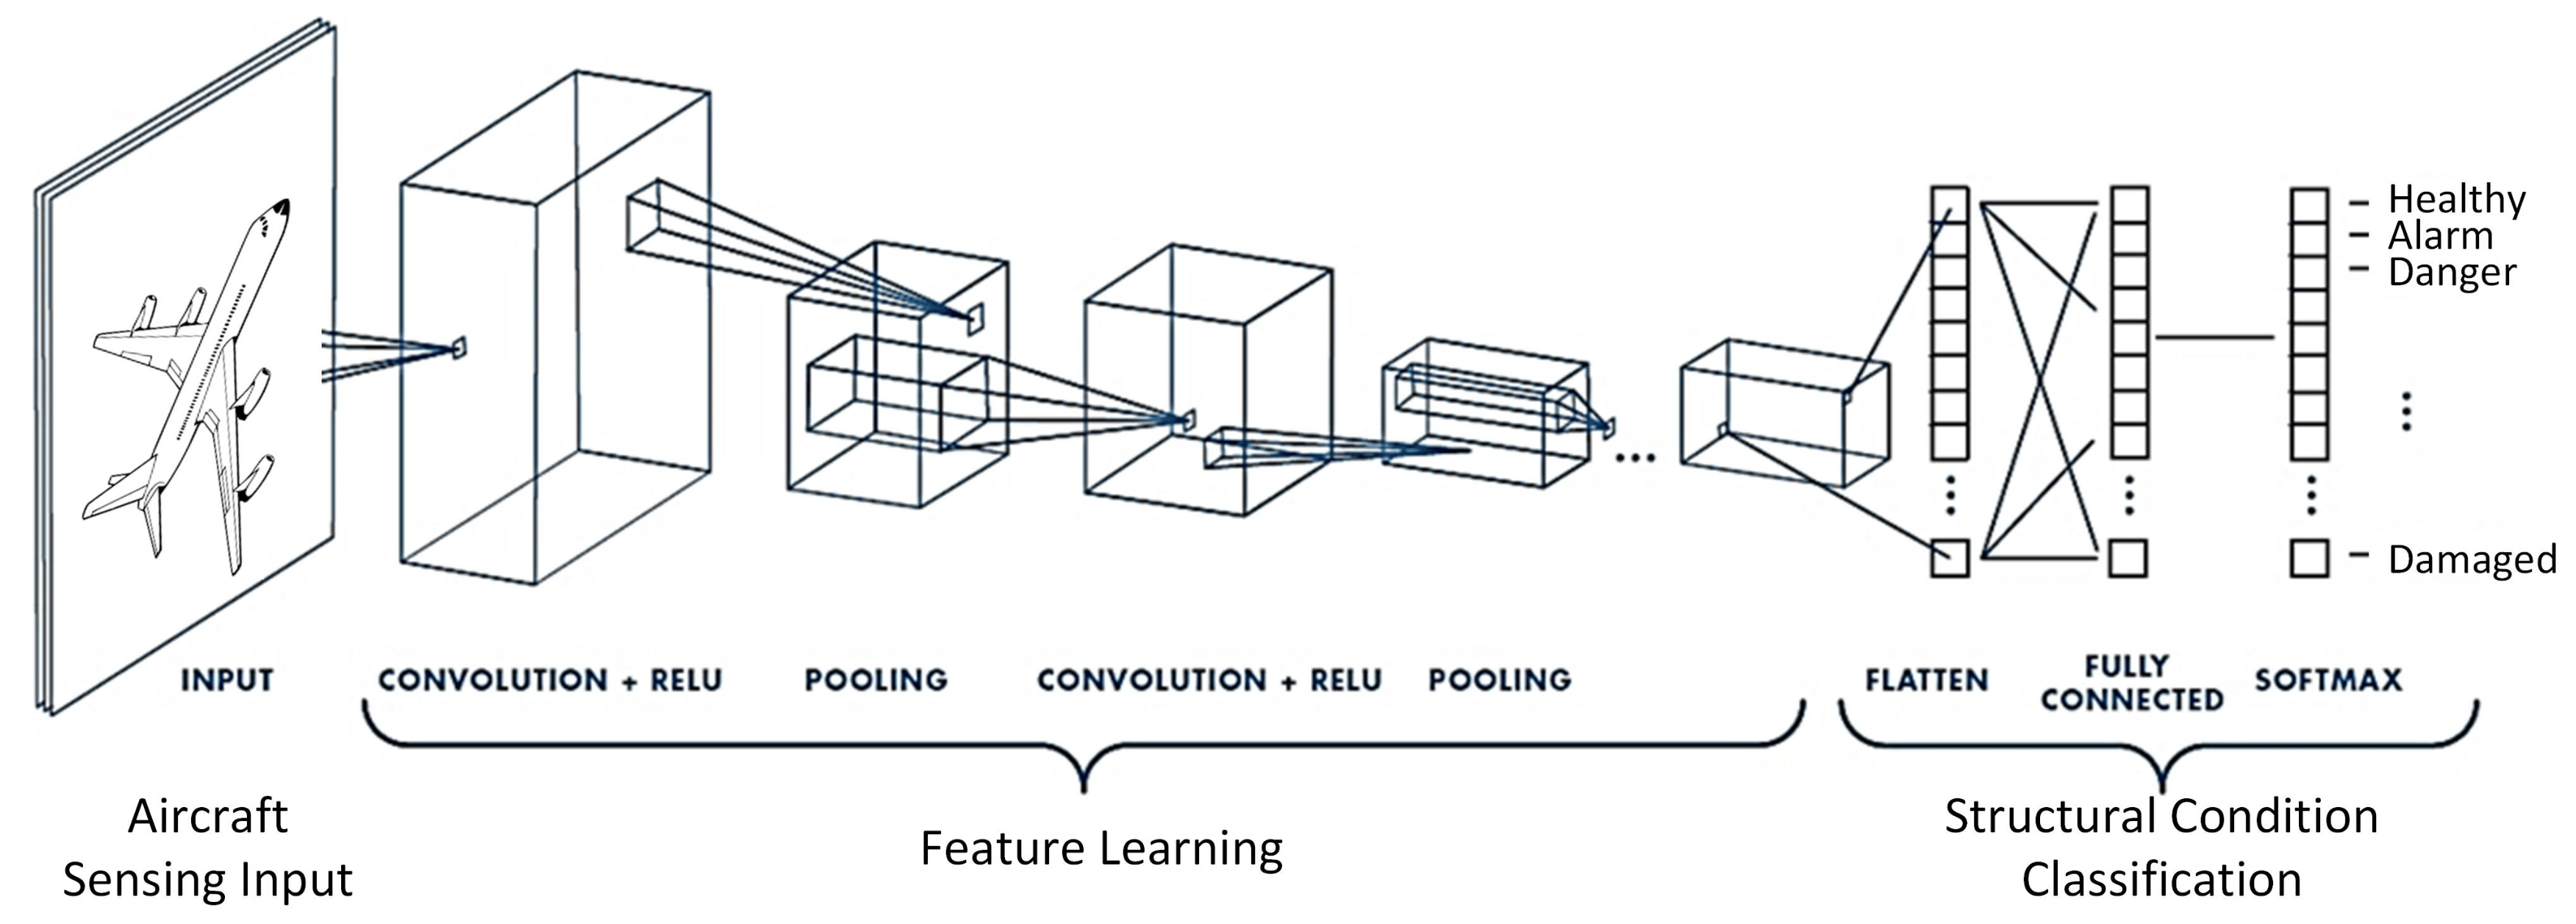
\includegraphics[scale=0.12]{gambar/arsitekturcnn.png}
    % Keterangan gambar yang diinputkan
    \caption{Arsitektur pada \emph{Convolutional Neural Network}}
    % Label referensi dari gambar yang diinputkan
    \label{fig:arsitektur cnn}
\end{figure}

Input CNN merupakan array tiga dimensi dengan ukuran seperti pada Persamaan \ref{eq:array3D}. Apabila input merupakan suatu citra maka citra tersebut harus diubah menjadi array dua dimensi. 

% Persamaan 2.1
\begin{equation}
    \label{eq:array3D}
    Baris * Kolom * Depth
\end{equation}

\emph{Convolution Layer} digunakan untuk menyaring (\emph{filter}) matriks dari citra \emph{input}. \emph{Zero Padd-ing} akan diperlukan untuk mempertahankan ukuran matriks dari citra \parencite{dwitama2019klasifikasi}. Ukuran kernel yang digunakan pada layer konvolusi adalah \(3 \times 3\) dan \(5 \times 5\). \emph{Output} dari lapisan konvolusi ini akan digunakan sebagai \emph{input} pada \emph{Pooling Layer} \parencite{hakim2018penerapan}. Apabila output dari \emph{Convolution Layer} bernilai negatif maka akan dilakukan perhitungan tambahan berupa aktifasi ReLU. Fungsi aktivasi ReLU akan nilai matriks yang bernilai negatif menjadi nol. Contoh penerapan dari aktivasi ReLU dapat dilihat pada Gambar \ref{fig:Aktivasi ReLU}.

% Gambar 2.2
\begin{figure} [ht] \centering
    % Nama dari file gambar yang diinputkan
    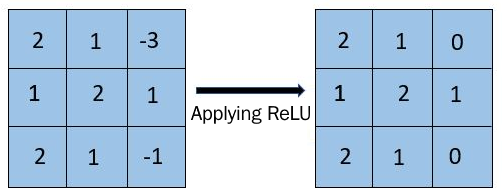
\includegraphics[scale=1]{gambar/aktivasiReLU.png}
    % Keterangan gambar yang diinputkan
    \caption{\emph{Aktivasi ReLU}}
    % Label referensi dari gambar yang diinputkan
    \label{fig:Aktivasi ReLU}
\end{figure}

\emph{Pooling Layer} digunakan untuk mengurangi jumlah parameter ketika ukuran citra terlalu besar dengan cara mengurangi dimensi setiap fitur. Karena ukuran citra menjadi lebih kecil maka proses \emph{feature map} akan menjadi lebih cepat \parencite{hakim2018penerapan}. \emph{Max Pooling} dilakukan dengan cara mengambil nilai dengan elemen terbesar sesuai dengan ukuran filter. Sebagai contoh pada Gambar \ref{fig:Max Pooling} merupakan \emph{max pooling} dengan filter \(2 \times 2\) dengan \emph{stride} sebesar 2.

% Gambar 2.3
\begin{figure} [ht] \centering
    % Nama dari file gambar yang diinputkan
    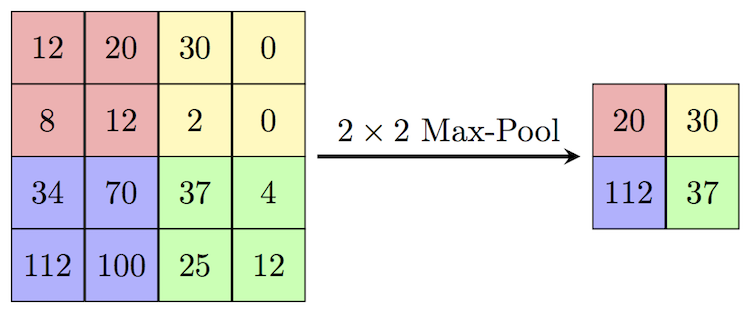
\includegraphics[scale=1.5]{gambar/maxPooling.png}
    % Keterangan gambar yang diinputkan
    \caption{\emph{Max Pooling}}
    % Label referensi dari gambar yang diinputkan
    \label{fig:Max Pooling}
\end{figure}

Flatten merupakan suatu proses dimana hasil dari \emph{Feature Learning} diubah menjadi vektor yang selanjutnya akan menjadi input pada proses klasifikasi dengan arsitektur \emph{fully connected layer}. Flatten digunakan untuk mengubah matriks menjadi vektor dengan menyesuaikan sesuai format \emph{input} pada \emph{neural network layer}. Flatten dapat digambarkan seperti pada Gambar \ref{fig:Proses Flattening}.

% Gambar 2.4
\begin{figure} [ht] \centering
    % Nama dari file gambar yang diinputkan
    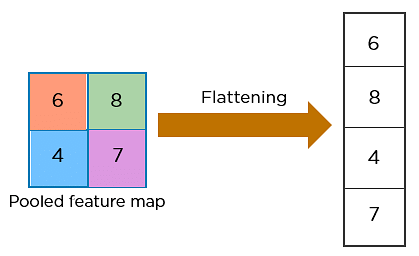
\includegraphics[scale=0.6]{gambar/flattening.png}
    % Keterangan gambar yang diinputkan
    \caption{Proses \emph{Flattening}}
    % Label referensi dari gambar yang diinputkan
    \label{fig:Proses Flattening}
\end{figure}

\subsection{Mediapipe}

MediaPipe merupakan \emph{framework} untuk membangun \emph{pipelines} yang dapat digunakan dalam melakukan pengambilan kesimpulan atau prediksi atas data sensorik. Dengan MediaPipe, sebuah \emph{perception pipeline} dapat dibangun sebagai grafik dari komponen modular termasuk inferensi model, algoritma pemrosesan media, serta transformasi data \parencite{lugaresi2019mediapipe}. MediaPipe menyediakan beragam solusi dari \emph{machine learning} seperti deteksi objek, klasifikasi citra, segmentasi citra, segmentasi interaktif, pengenalan gestur, deteksi \emph{landmark} tangan, deteksi wajah, deteksi \emph{landmark} wajah, deteksi pose, klasifikasi teks, penyematan teks, deteksi bahasa hingga klasifikasi suara.

Keunggulan dari menggunakan MediaPipe adalah dari fleksibilitas yang dimiliki oleh \emph{fra-mework} ini. MediaPipe telah dikembangkan menggunakan bahasa pemrograman C++ sebagai bahasa inti. Namun MediaPipe juga menyediakan berbagai ikatan bahasa pemrograman yang lain seperti Python dan Java. Hal ini membuatnya dapat digunakan pada berbagai lingkungan pengembangan. Sehingga MediaPipe dapat diintegrasikan pada berbagai projek pengembangan dengan berbagai bahasa pemrograman.

Kemampuan MediaPipe yang dapat berjalan pada berbagai platform merupakan terobosan yang sangat membantu para pengembang. MediaPipe dapat berjalan pada perangkat seluler, desktop hingga lingkungan cloud. Sehingga para pengembang dapat menerapkan berbagai solusi MediaPipe pada berbagai skenario dan perangkat tanpa perlu membatasi diri pada suatu platform tertentu.

Komponen-komponen untuk mengestimasi tangan manusia sudah tersedia pada MediaPipe dalam video maupun aliran gambar. MediaPipe dapat mengenali posisi dan orientasi berbagai bagian tangan manusia, baik pergelangan tangan hingga ruas-ruas setiap jari yang dapat dilihat pada Gambar \ref{fig:handLandmark}. Dengan kemampuan tersebut maka MediaPipe dapat mengidentifikasi pola-pola khusus yang berkaitan dengan aktivitas yang kompleks seperti menerjemah bahasa isyarat.

\begin{figure} [ht] \centering
    % Nama dari file gambar yang diinputkan
    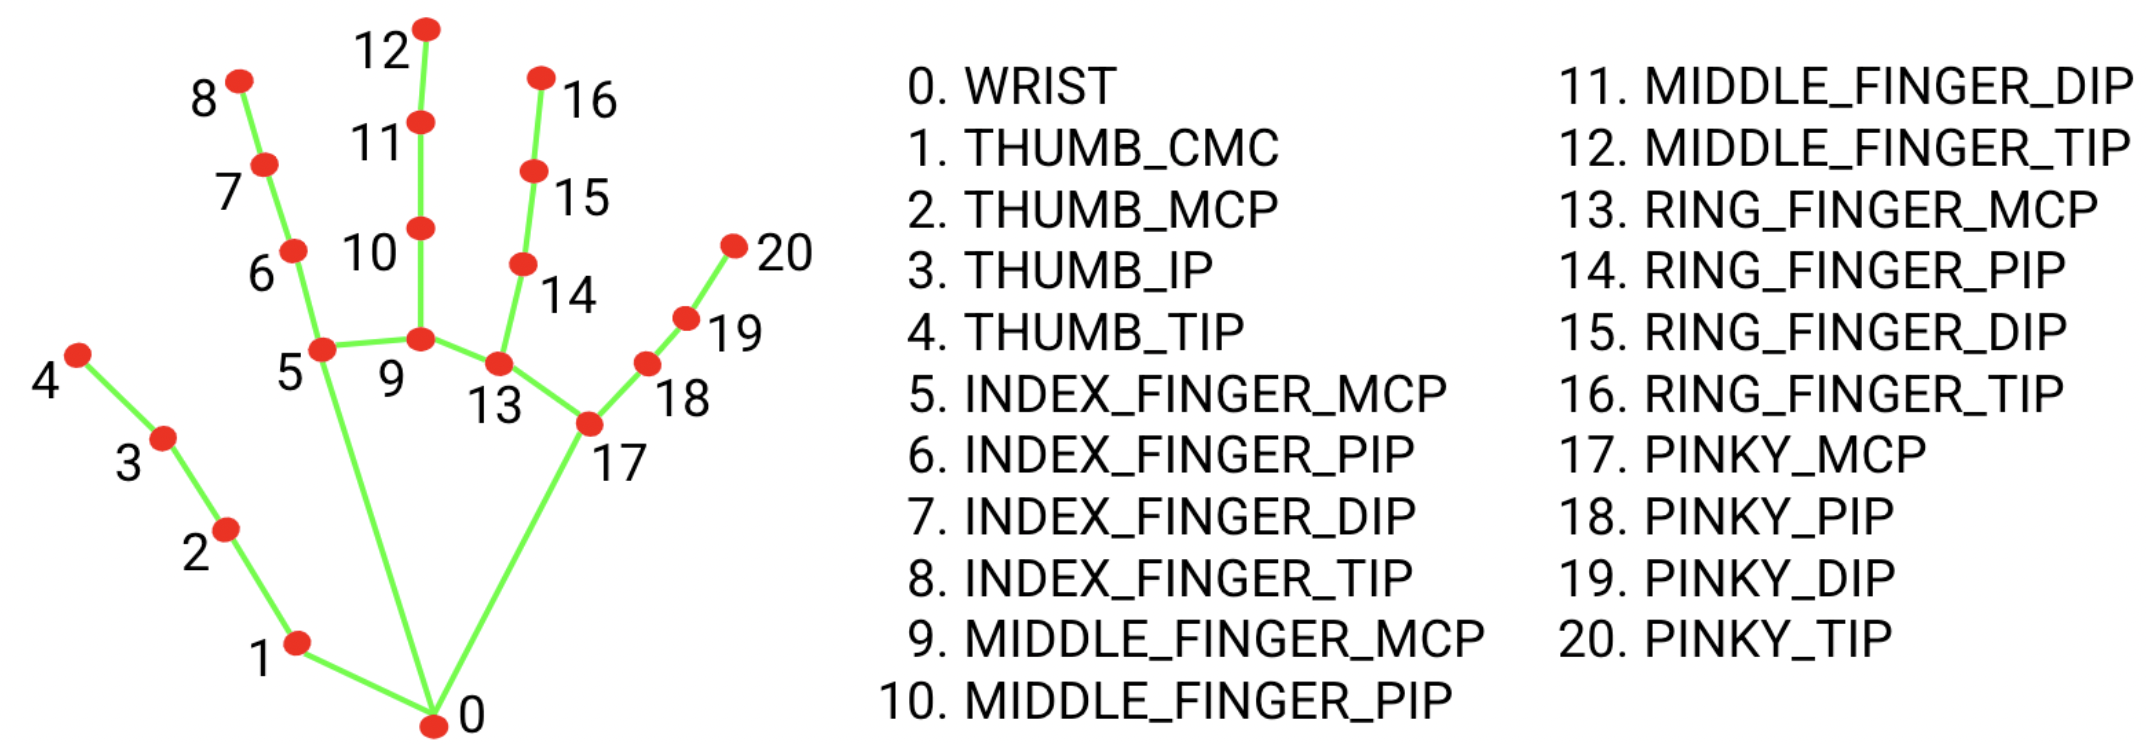
\includegraphics[scale=0.4]{gambar/handLandmark.png}
    % Keterangan gambar yang diinputkan
    \caption{\emph{Landmark} Tangan Manusia Pada MediaPipe}
    % Label referensi dari gambar yang diinputkan
    \label{fig:handLandmark}
\end{figure}
\newpage

\subsection{TensorFlow} 

\begin{figure} [ht] \centering
    % Nama dari file gambar yang diinputkan
    
\includegraphics[scale=0.65]{gambar/TensorflowLogo.png}
    % Keterangan gambar yang diinputkan
    \caption{Logo TensorFlow}
    % Label referensi dari gambar yang diinputkan
    \label{fig:TensorflowLogo}
\end{figure}

TensorFlow merupakan platform \emph{open source} untuk \emph{machine learning}. TensorFlow memiliki fitur untuk menjalankan \emph{training} model menggunakan \emph{Central Processing Unit} (CPU) dan \emph{training} model \emph{Graphic Processing Unit} (GPU) yang memiliki waktu \emph{training} yang lebih cepat dibanding \emph{training} model CPU \parencite{nurfita2018implementasi}.

TensorFlow awalnya dikembangkan oleh para peneliti dan pengembang yang bekerja sebagai tim \emph{Machine Learning} di Google Brain untuk melakukan penelitian di bidang \emph{machine learning} dan \emph{neural network}. \emph{Framework} ini dirilis pertama kali pada bulan Februari 2017 dan terus dikembangkan hingga sekarang\parencite{Developers_2021}.

\subsection{Arduino IDE}

Arduino Integrated Development Environment (IDE) merupakan perangkat lunak sumber terbuka yang digunakan untuk menulis dan mengunggah kode ke mikrokontroler seperti Arduino maupun ESP buatan Espressif System. Arduino IDE berisikan editor teks untuk menulis kode program, toolbar dengan tombol untuk fungsi umum serta serangkaian menu. Program yang ditulis menggunakan Arduino IDE disebut sketches. Sketches ditulis 
pada teks editor dan disimpan pada file dengan ekstensi .ino. Editor memiliki fitur untuk memotong dan menempel serta untuk mencari dan mengganti teks. Area pesan akan memberikan umpan balik ketika menyimpan dan mengekspor serta akan menampilkan error. Konsol menampilkan keluaran teks oleh Arduino IDE termasuk pesan error yang lengkap serta informasi lainnya \parencite{Söderby_Hylén_2023a}.

\begin{figure} [ht] \centering
    % Nama dari file gambar yang diinputkan
    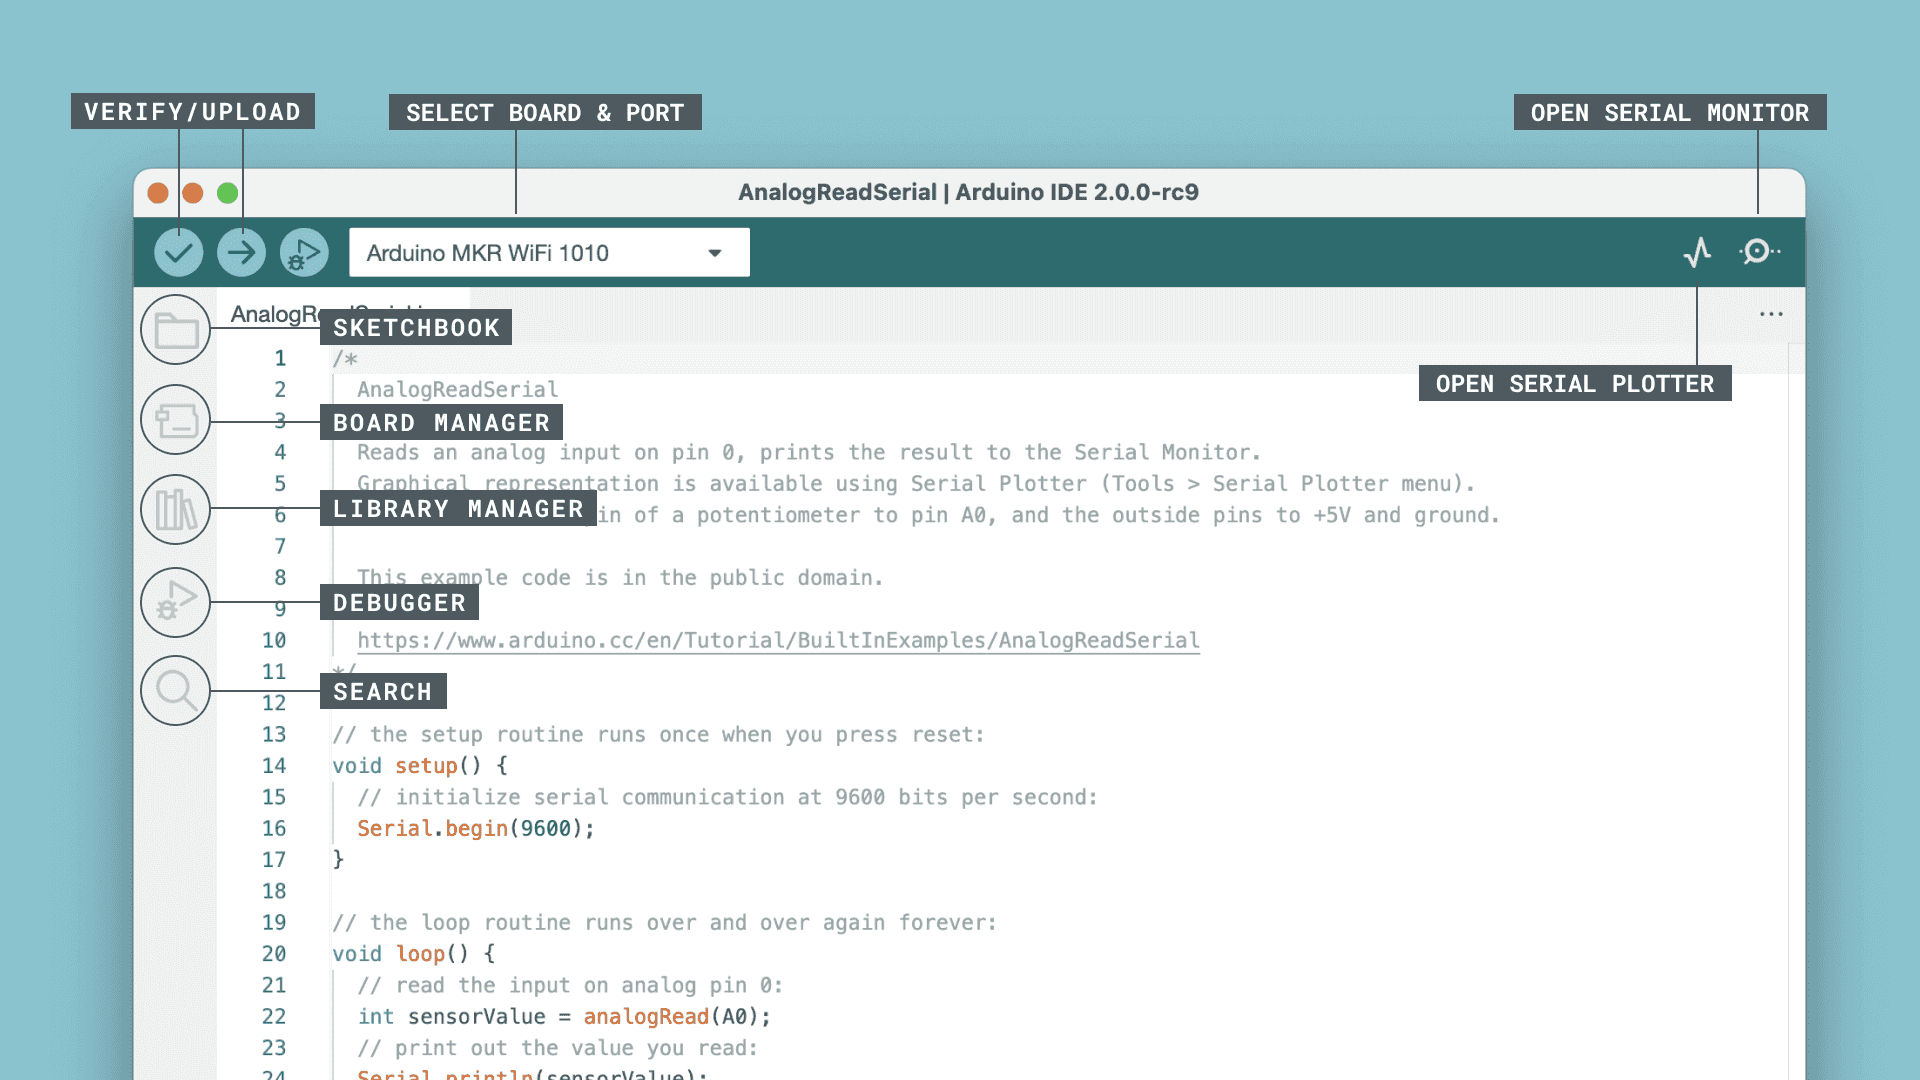
\includegraphics[scale=0.235]{gambar/arduinoIDEoverview.png}
    % Keterangan gambar yang diinputkan
    \caption{Tampilan Arduino IDE 2}
    % Label referensi dari gambar yang diinputkan
    \label{fig:ArduinoIDEOverview}
\end{figure}

Gambar \ref{fig:ArduinoIDEOverview} merupakan tampilan dari Arduino IDE. Arduino IDE 2 dilengkapi dengan \emph{sidebar} baru yang memudahkan pengguna dalam mengakses \emph{tools} yang umum digunakan. \emph{Verify/Upload} digunakan untuk \emph{compile} dan \emph{upload} program ke \emph{Board} Arduino. \emph{Select Board} \& \emph{Port} digunakan untuk mendeteksi \emph{Board} Arduino beserta nomor port yang terhubung dengan Arduino. \emph{Sketchbook} merupakan tempat untuk mencari semua \emph{sketchbook} lokal yang disimpan pada komputer pengguna. Sebagai tambahan, pengguna dapat menguhubungkan Arduino IDE dengan Arduino Cloud sehingga pengguna dapat menyimpan \emph{sketch} pada lingkungan daring. \emph{Board Manager} merupakan kumpulan \emph{board} arduino serta \emph{board packages} pihak ketiga yang dapat diinstal \parencite{Söderby_Hylén_2023b}. \emph{Library Manager} merupakan tempat untuk menginstal berbagai \emph{library} yang mendukung pengembangan Arduino, baik yang dibuat oleh Arduino maupun dari komunitas \parencite{Söderby_Hylén_2023c}. \emph{Debugger} berguna untuk menguji dan men-\emph{debug} program secara \emph{realtime}. \emph{Search} digunakan untuk mencari kata kunci pada program yang sedang dimuat. \emph{Open Serial Monitor} berguna untuk memuat Serial Monitor yang sangat berguna untuk pengembangan \parencite{Söderby_2023}.

\emph{Sketchbook} merupakan tempat dimana file program akan disimpan. \emph{Sketches} Arduino akan disimpan dengan tipe file .ino dan harus disimpan pada folder dengan nama folder yang sama dengan nama file. Sebagai contoh, file my\_sketch.ino harus disimpan pada folder dengan nama folder my\_sketch.

Dengan menggunakan \emph{Library Manager}, pengguna dapat menemukan dan menginstal ribuan \emph{library} yang dapat membantu dalam mengembangkan proyek menggunakan . \emph{Library} merupakan \emph{extension} dari Arduino API yang dapat memudahkan pengembang. Sebagai contoh, para pengembang dapat mengontrol motor servo, membaca sensor tertentu, hingga menggunakan modul WiFi hanya dengan memanggil fungsi yang terdapat pada \emph{library} \parencite{Söderby_Hylén_2023c}.

\emph{Serial Monitor} merupakan alat yang memungkinkan pengguna untuk melihat \emph{streaming} data pada \emph{Board} Arduino yang terhubung. Pada Arduino versi 1, \emph{tool} ini ditempatkan pada jendela yang terpisah, namun untuk memudahkan pengguna maka \emph{tool} ini kini terintegrasi dengan editor \parencite{Söderby_2023}. 

\subsection{Anaconda® Distribution}

Anaconda® merupakan distribusi Python yang berisi conda yang merupakan manajer paket dan lingkungan pengembangan dengan menggunakan CLI (\emph{Command Line Interface}), Anaconda Navigator yang merupakan aplikasi desktop yang dibangun diatas conda, hingga akses ke Anaconda \emph{Public Repository} \parencite{Inc_2018}.

\begin{figure} [ht] \centering
    % Nama dari file gambar yang diinputkan
    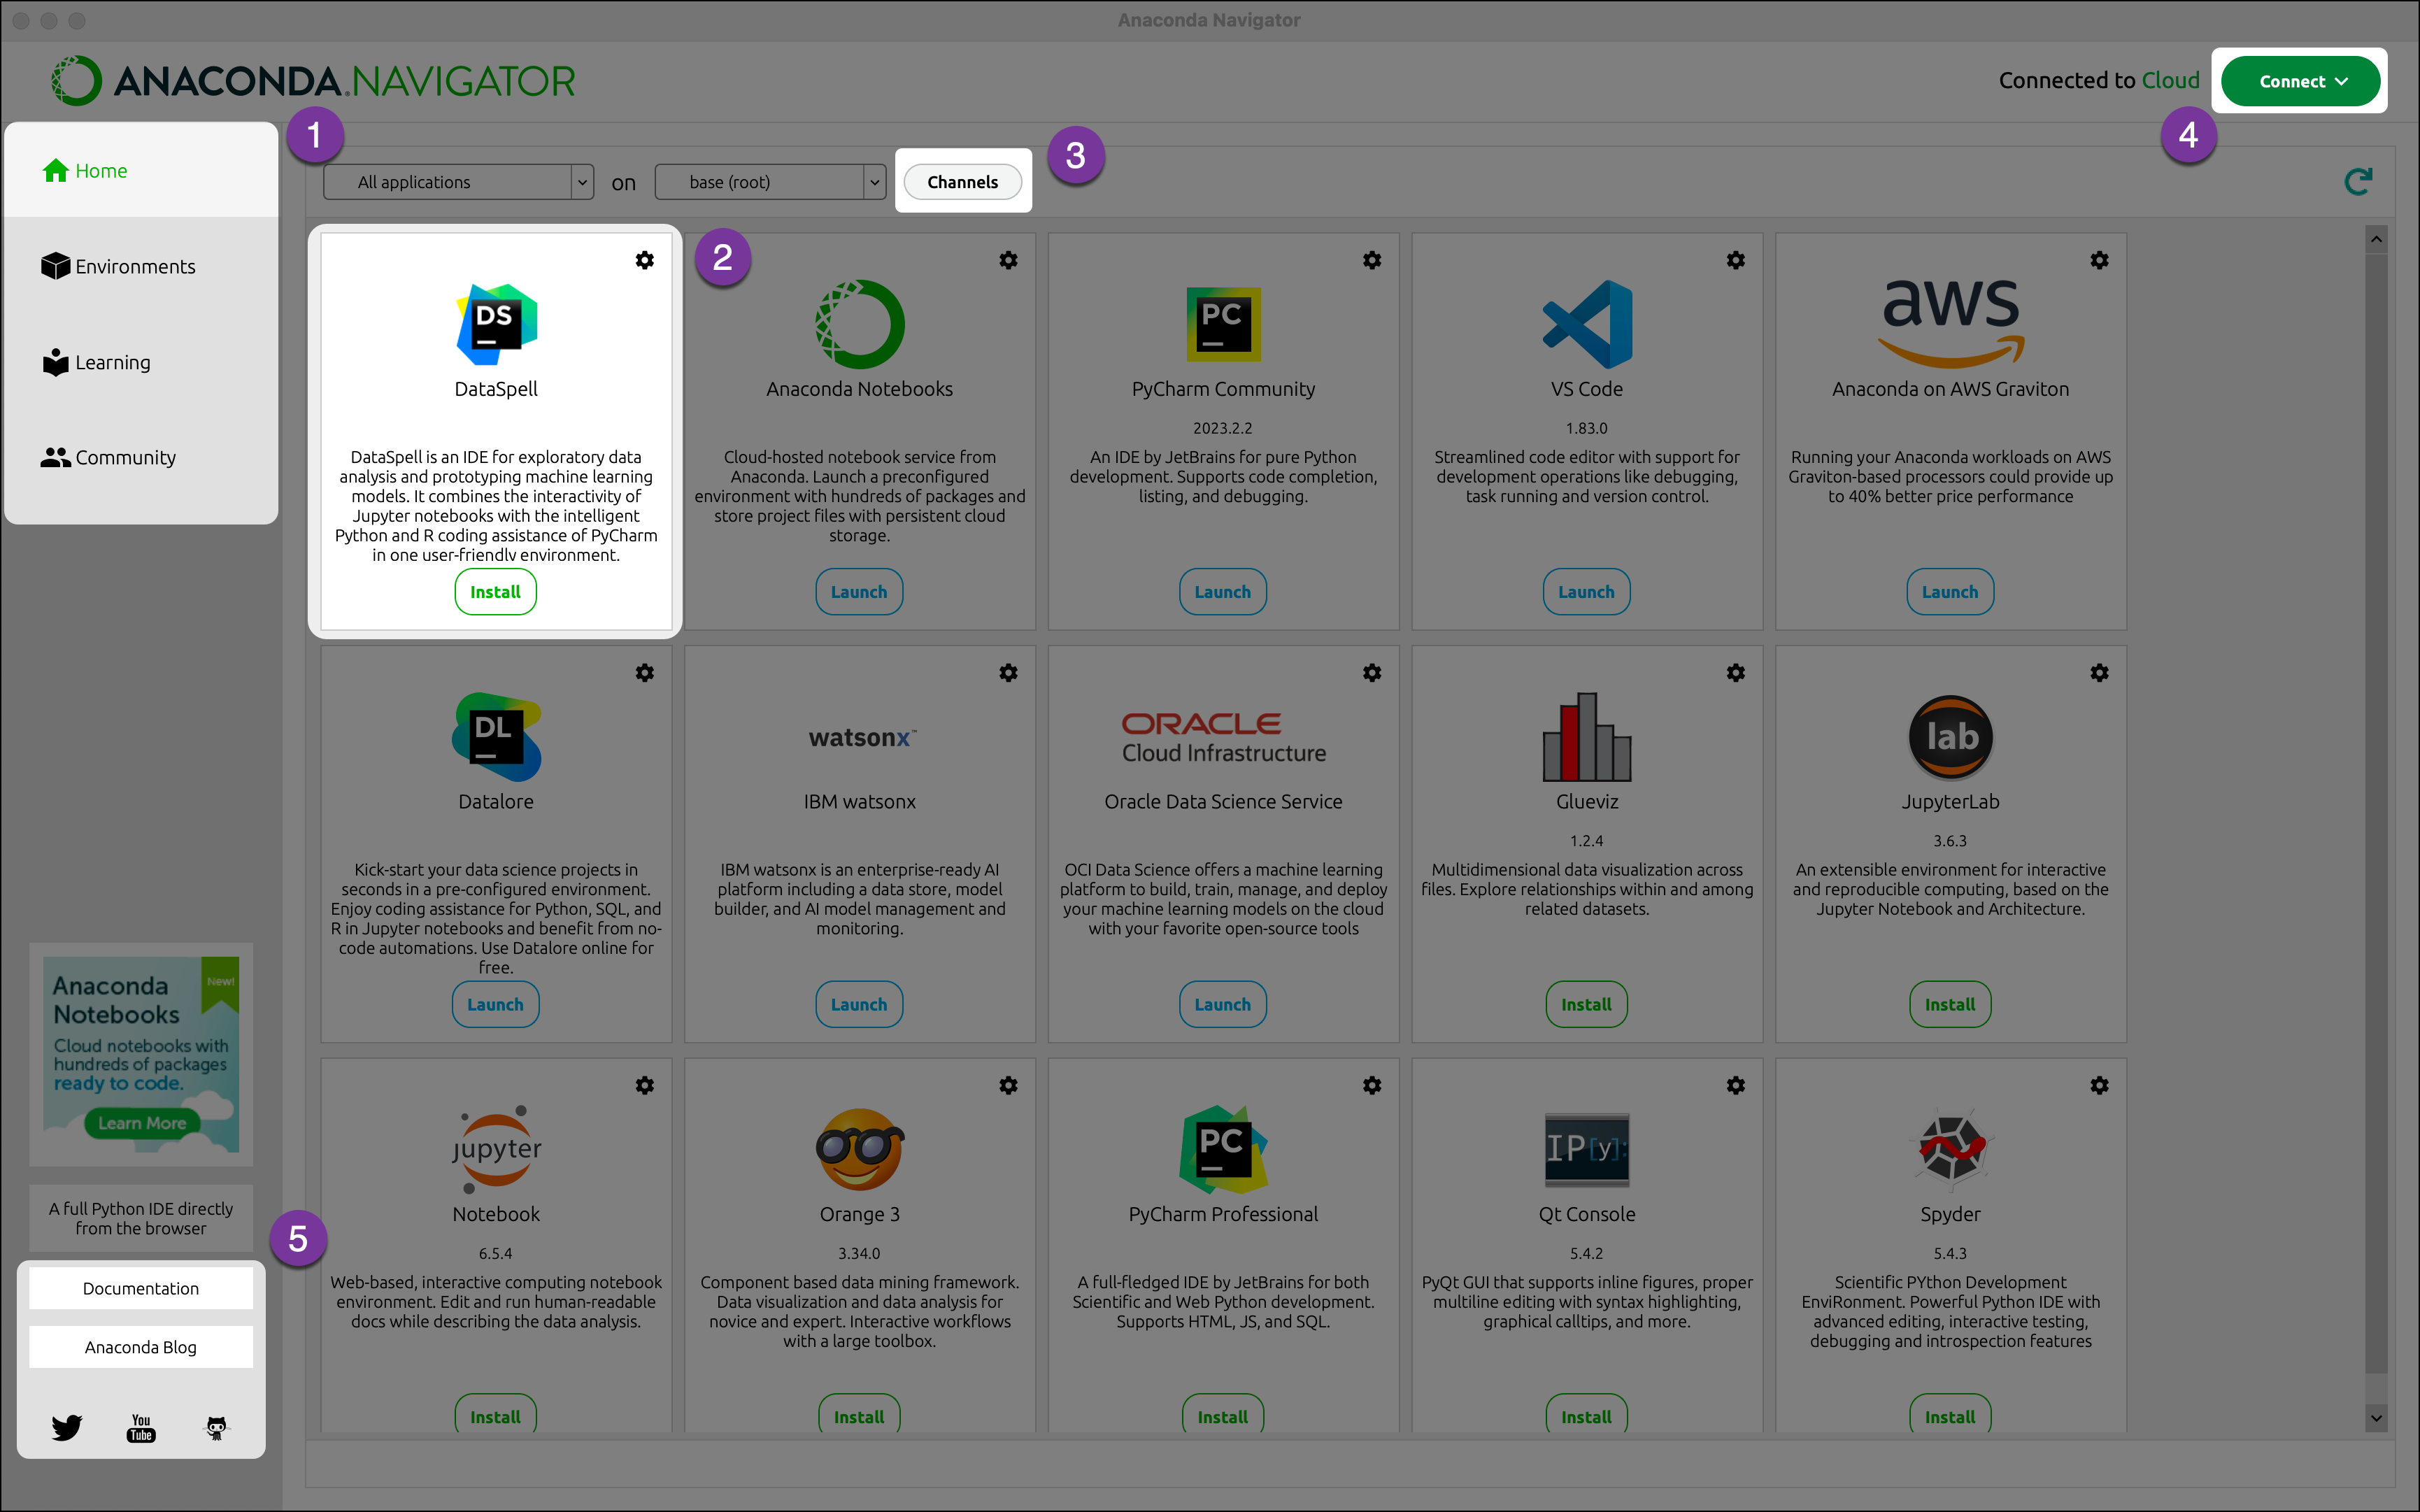
\includegraphics[scale=0.262]{gambar/AnacondaNavigatorOverview.png}
    % Keterangan gambar yang diinputkan
    \caption{Tampilan Anaconda Navigator}
    % Label referensi dari gambar yang diinputkan
    \label{fig:Tampilan Anaconda Navigator}
\end{figure}

Tampilan utama pada Anaconda Navigator dapat dilihat pada Gambar \ref{fig:Tampilan Anaconda Navigator}. \emph{Navigator Pages} yang ditandai dengan nomor 1 digunakan untuk mengakses halaman utama. Halaman utama akan secara otomatis terbuka ketika pertama kali membuka aplikasi Anaconda Navigator. \emph{Application/Package Tile} ditandai dengan nomor 2 yang digunakan untuk menginstal atau menjalankan aplikasi Python yang dapat berjalan didalam lingkungan Anaconda. \emph{Channels} ditandai dengan nomor 3 digunakan untuk mencari dan menginstal paket. \emph{Connect} yang ditandai dengan nomor 4 digunakan untuk menghubungkan Anaconda Navigator dengan Anaconda Cloud. Masuk ke layanan repositori akan memungkinkan pencarian paket dalam repositori itu. \emph{Outside Links} yang ditandai dengan nomor 5 digunakan untuk mengunjungi dokumentasi, blog, serta sosial media resmi Anaconda.

\begin{figure} [ht] \centering
    % Nama dari file gambar yang diinputkan
    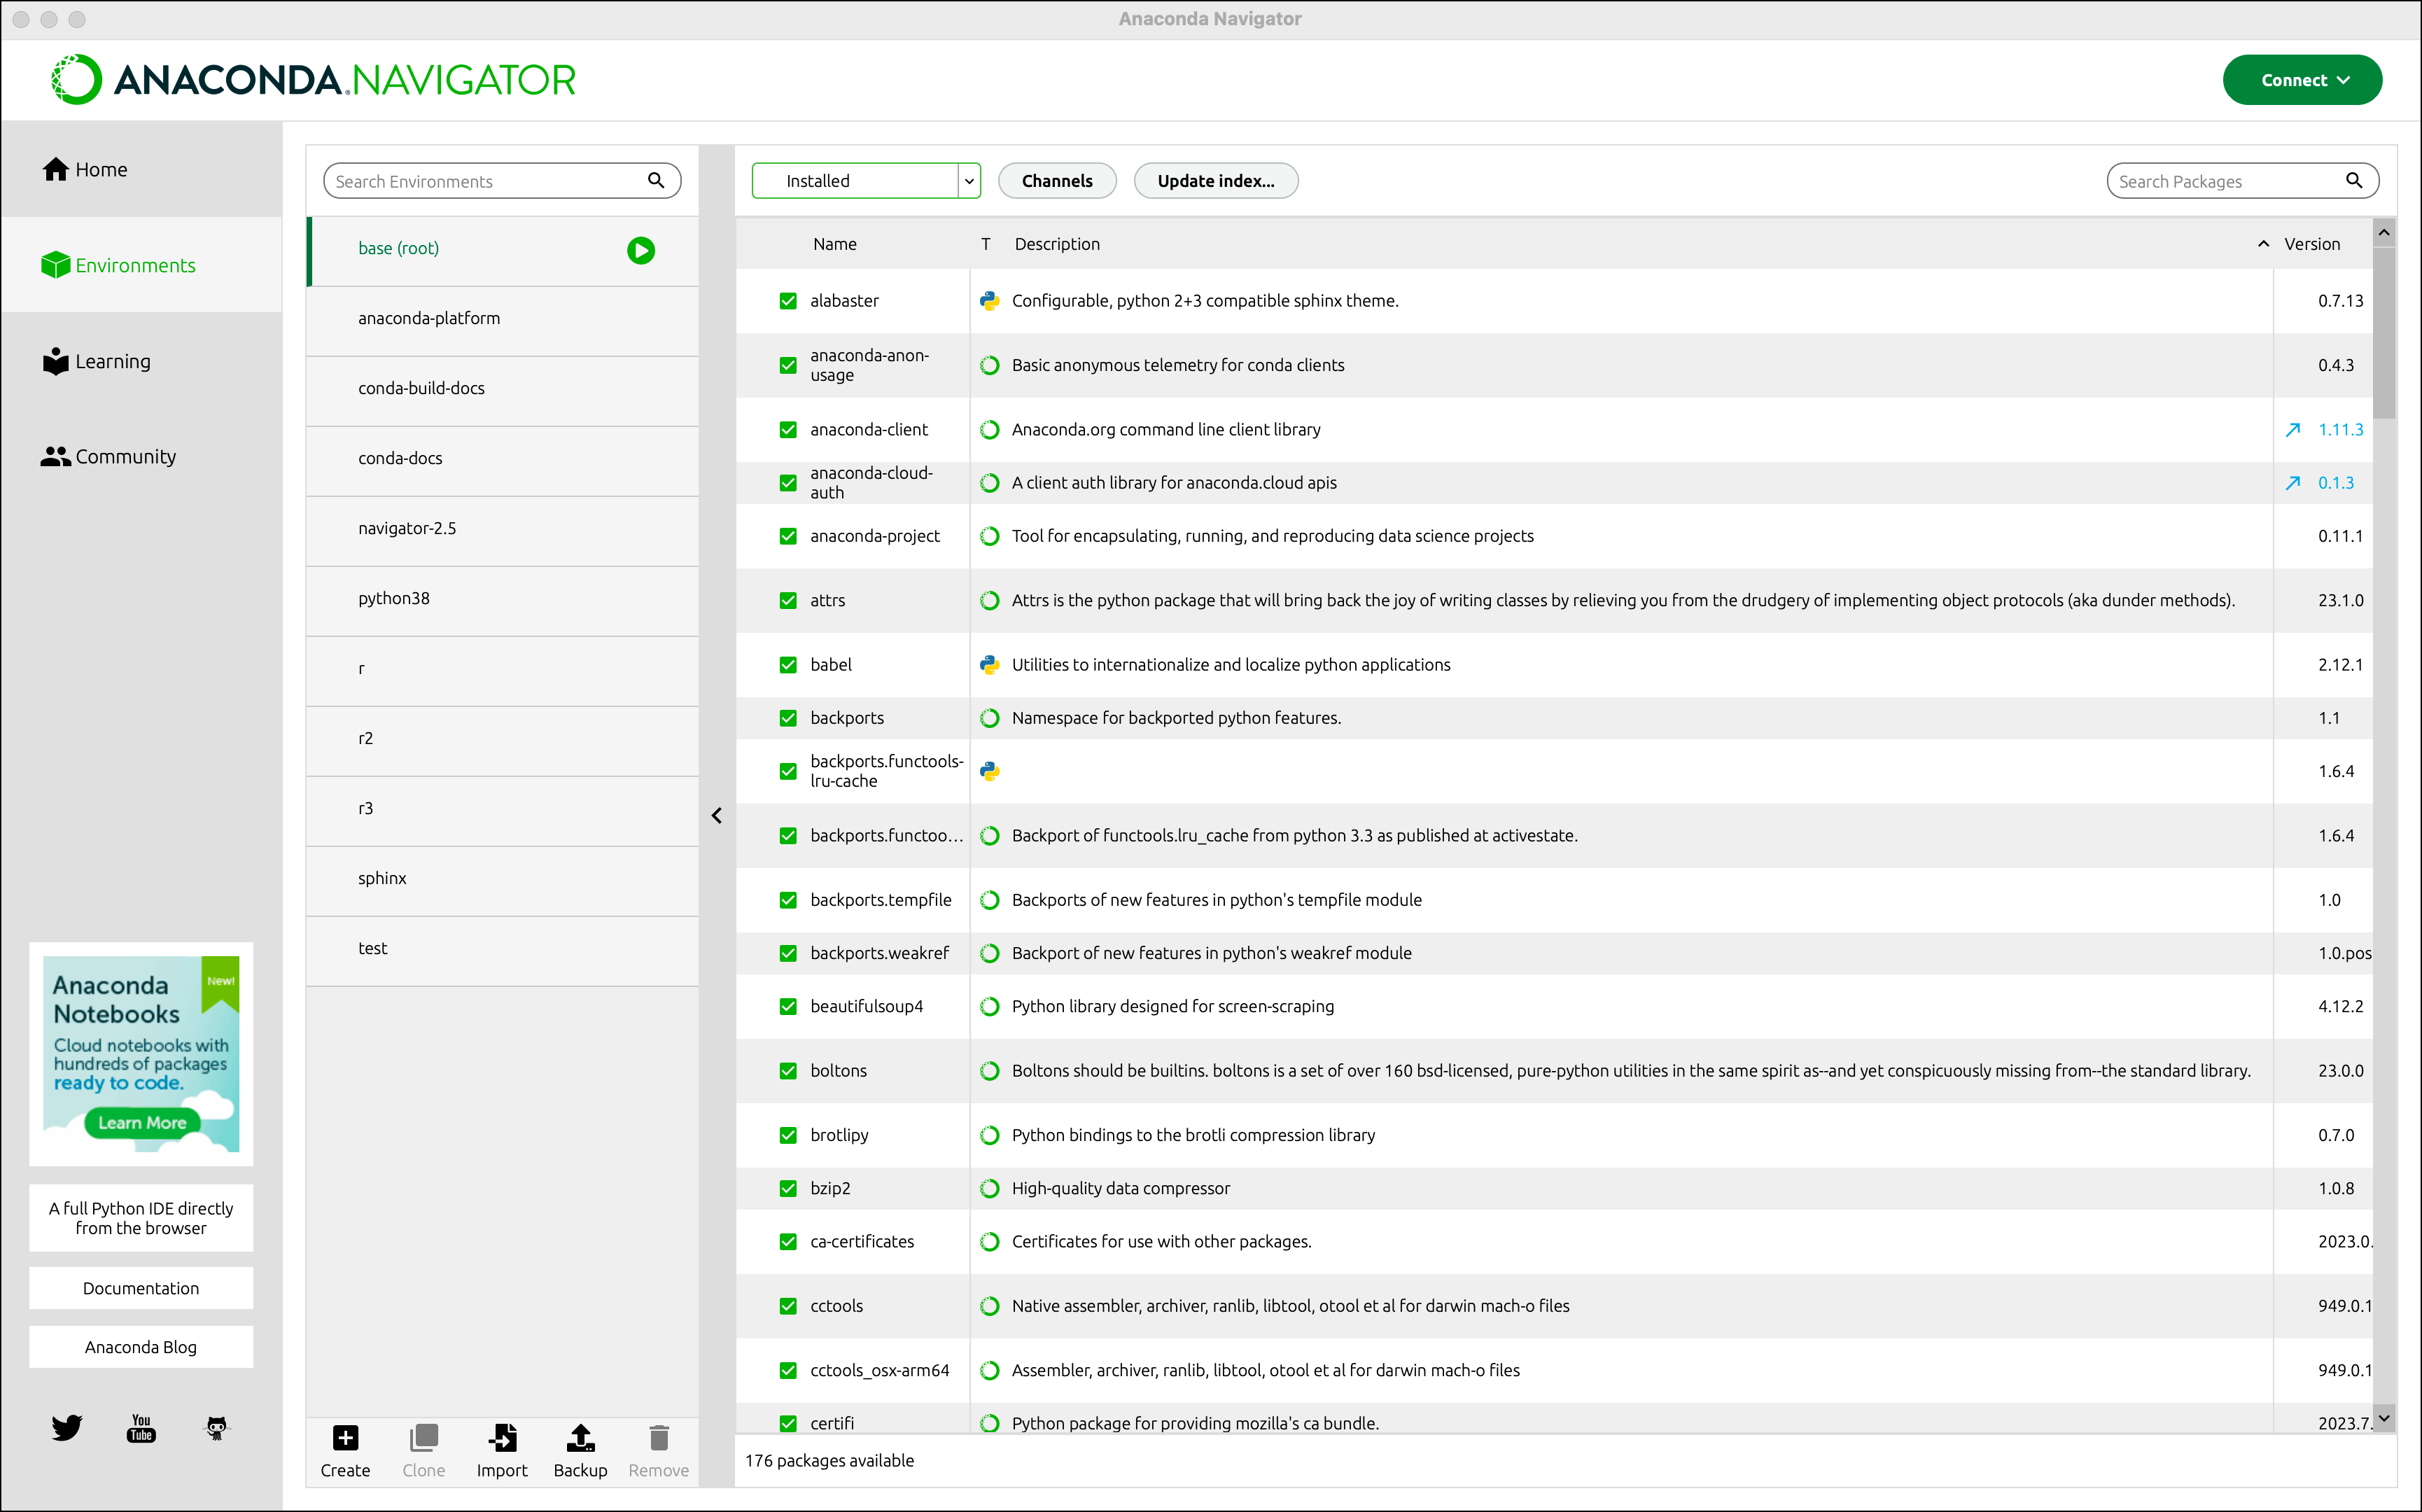
\includegraphics[scale=0.262]{gambar/AnacondaEnvironments.png}
    % Keterangan gambar yang diinputkan
    \caption{Tampilan Halaman \emph{Environments} pada Anaconda Navigator}
    % Label referensi dari gambar yang diinputkan
    \label{fig:Tampilan Anaconda Environments}
\end{figure}

Tampilan halaman \emph{environments} pada Anaconda Navigator dapat dilihat pada Gambar \ref{fig:Tampilan Anaconda Environments}. Halaman \emph{environments} memungkinkan pengguna untuk mengelola \emph{environment}, \emph{package}, dan \emph{channel}. Pada kolom kiri terdapat daftar dari \emph{environment} yang dibuat oleh pengguna. Dengan menggunakan Navigator maka pengguna dapat membuat, mengekspor, membuat daftar, menghapus, dan memperbaharui \emph{environments} dengan versi Python serta \emph{packages} yang berbeda. Pada kolom kanan terdapat daftar dari \emph{packages} yang terinstal maupun yang dapat diinstal. Tampilan \emph{default}nya adalah \emph{packages} yang terinstal. Untuk melihat daftar \emph{packages} lainnya pengguna dapat memilih daftar \emph{Installed, Not Installed, Updatable, Selected,} serta \emph{All Packages}. \emph{Channels} merupakan tempat dimana Navigator maupun conda mencari \emph{packages}.

\subsection{JupyterLab}

JupyterLab merupakan \emph{environment} pengembangan yang dirancang untuk analisis data, komputasi ilmiah, hingga pengembangan proyek menggunakan Python maupun R. JupyterLab masih menjadi bagian dari Proyek Jupyter yang terpusat dengan tujuan untuk menyediakan layanan komputasi interaktif dengan \emph{notebooks} yang terkomputasi \parencite{Jupyter_2023}. 

\emph{Computational Notebook} atau \emph{notebook} yang terkomputasi merupakan suatu dokumen yang dapat dibagikan kepada pengguna lain yang menggabungkan kode komputer, deskripsi kode, data, visualisasi data seperti 3D Model, grafik, diagram, gambar, hingga kontrol yang interaktif \parencite{Team_2015}. Suatu \emph{notebook}, bersamaan dengan editor seperti JupyterLab, menyediakan \emph{environment} interaktif untuk mengembangkan prototipe, menjelaskan kode, mengeksplorasi serta memvisualisasi data. 

\newpage
\begin{figure} [ht] \centering
    % Nama dari file gambar yang diinputkan
    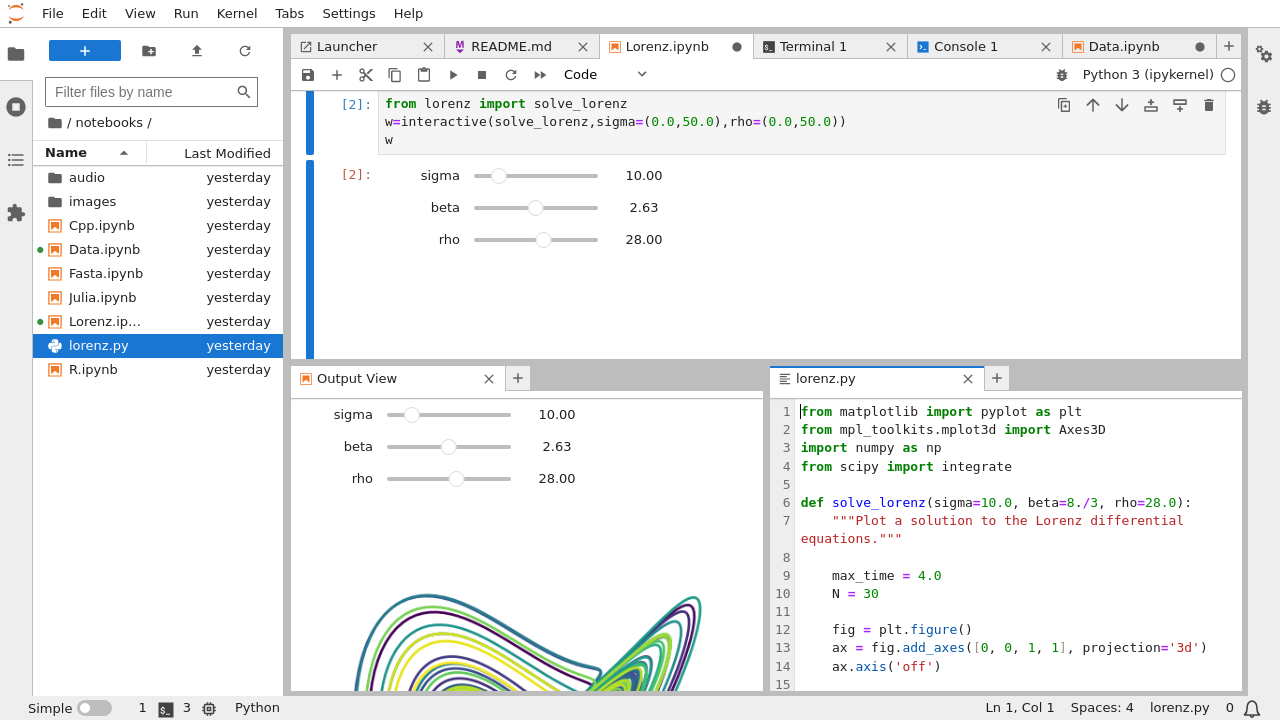
\includegraphics[scale=0.35]{gambar/JupyterLab.png}
    % Keterangan gambar yang diinputkan
    \caption{Tampilan Halaman pada JupyterLab}
    % Label referensi dari gambar yang diinputkan
    \label{fig:JupyterLab}
\end{figure}

Gambar \ref{fig:JupyterLab} merupakan tampilan utama dari JupyterLab. JupyterLab akan berjalan pada browser pengguna karena sifatnya yang \emph{web-based} \parencite{Jupyter_2023b}. JupyterLab memungkinkan pengguna untuk bekerja dengan dokumen pada Jupyter Notebook, editor teks, terminal, serta komponen kustom secara fleksibel, terintegrasi dan dapat diperluas. Pengguna dapat mengatur beberapa dokumen dan aktivitas secara berdampingan pada area kerja menggunakan tab dan pemisah. Dokumen serta aktivitas akan terintegrasi antara satu dengan yang lainnya sehingga memungkinkan untuk melakukan alur kerja baru dengan komputasi yang interaktif.

\subsection{NVIDIA® Jetson Nano™}

\begin{figure} [ht] \centering
    % Nama dari file gambar yang diinputkan
    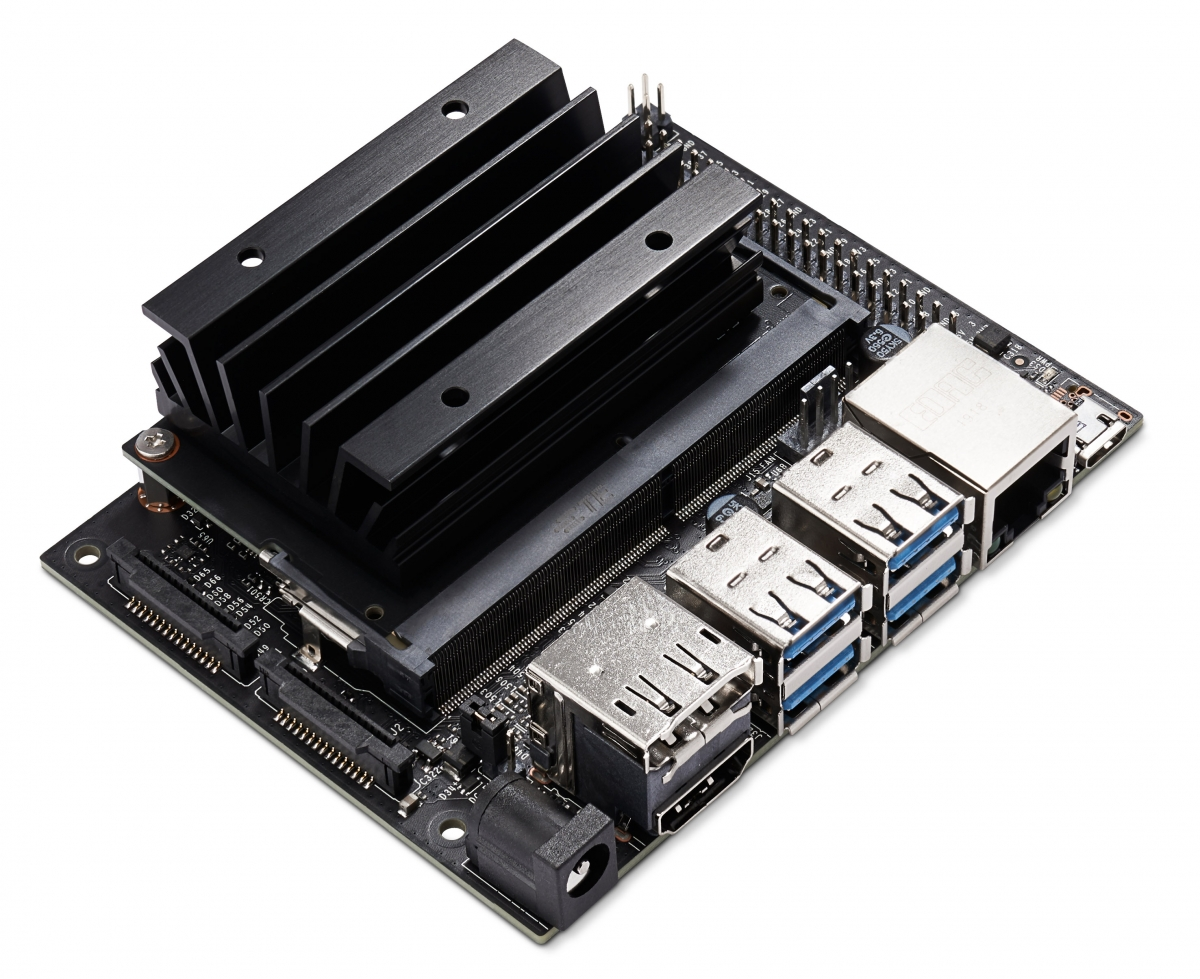
\includegraphics[scale=0.25]{gambar/JetsonNano.jpg}
    % Keterangan gambar yang diinputkan
    \caption{Perangkat Jetson Nano}
    % Label referensi dari gambar yang diinputkan
    \label{fig:Perangkat Jetson Nano}
\end{figure}

NVIDIA® Jetson Nano™ Developer Kit adalah komputer kecil dan kuat yang dapat digunakan untuk menjalankan beberapa \emph{neural network} secara paralel untuk berbagai penerapan seperti klasifikasi gambar, deteksi objek, segmentasi, dan pemrosesan ucapan. Semuanya dikemas dalam platform yang mudah digunakan dan hanya membutuhkan daya 5 watt \parencite{Developer_2023}.

Perangkat ini memiliki pin \emph{input} serta \emph{output} yang berlimpah, mulai dari GPIO hingga pin CSI. Jumlah pin yang berlimpah ini sangat memudahkan para pengembang dalam menghubung-kan berbagai perangkat tambahan seperti sensor untuk keperluan pengembangan aplikasi \emph{Artificial Intelligence}. NVIDIA® Jetson Nano™ Developer Kit juga didukung dengan NVIDIA JetPack yang mencakup berbagai perangkat lunak seperti Sistem Operasi Linux, cuDNN, NVIDIA CUDA, TensorRT, dan juga \emph{Board Support Package} (BSP) yang digunakan untuk keperluan \emph{Deep Learning} serta visi komputer.

\subsection{ESP32 Devkit V1}

\begin{figure} [ht] \centering
    % Nama dari file gambar yang diinputkan
    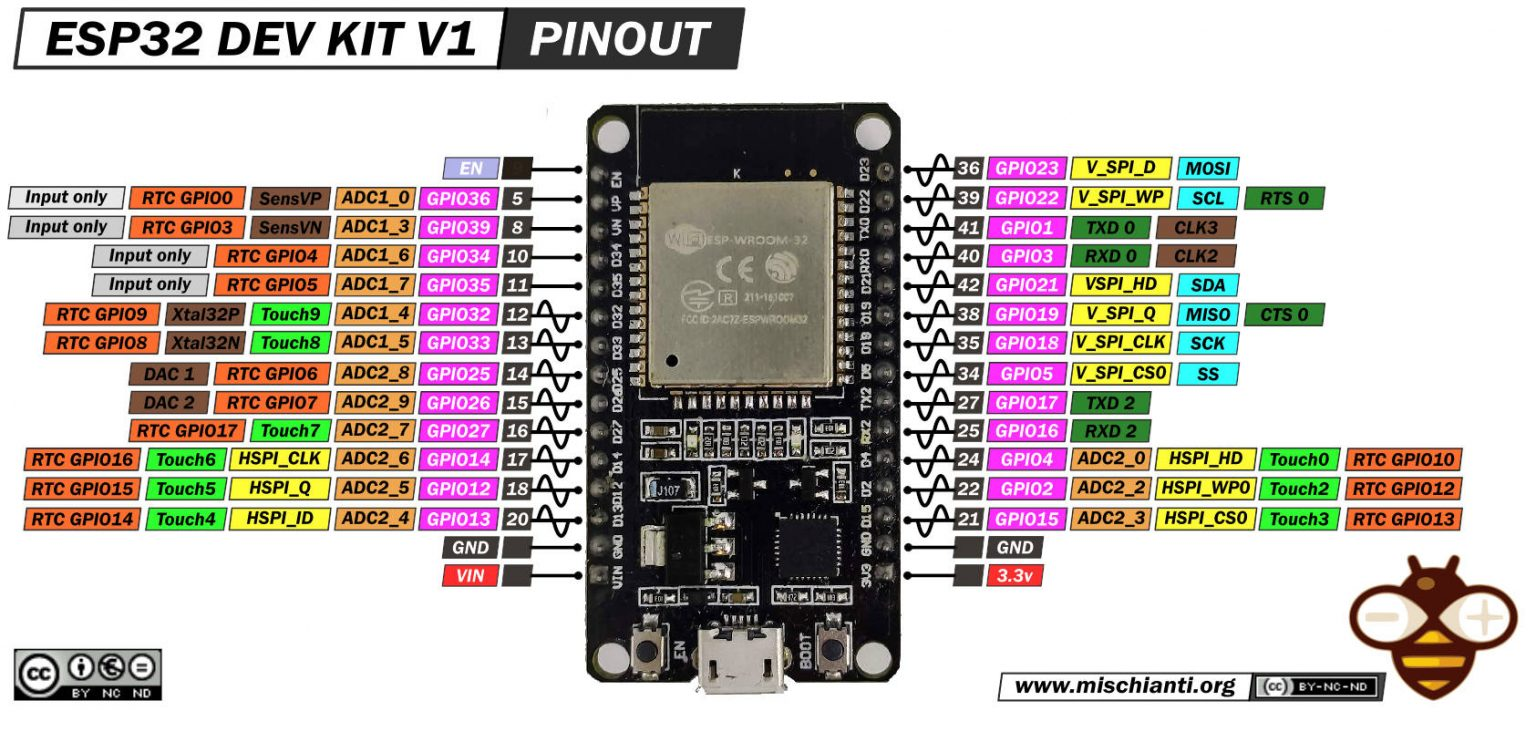
\includegraphics[scale=0.39]{gambar/ESP32DevkitV1.jpg}
    % Keterangan gambar yang diinputkan
    \caption{Perangkat ESP32 Devkit V1}
    % Label referensi dari gambar yang diinputkan
    \label{fig:Perangkat ESP32}
\end{figure}

ESP32 Devkit V1 merupakan salah satu \emph{development board} yang dibuat oleh DOIT untuk menjalankan modul ESP-WROOM-32 buatan Espressif \parencite{SmartArduino_2022}. \emph{Development Board} ini berisi WiFi, Bluetooth, serta berdaya rendah hanya dengan 1 chip. Setiap pin dari ESP32 Devkit V1 dapat dilihat pada Gambar \ref{fig:Perangkat ESP32}. Flash internal modul ESP32 disusun dalam satu area flash dengan 4096 \emph{byte} pada masing-masing halaman. Alamat flash dimulai dari 0x00000.

Daya untuk menjalankan ESP32 disuplai melalui konektor Micro USB Tipe B atau dapat langsung melalui pin "VIN". Perangkat dapat beroperasi pada tegangan antara 6 Volt hingga 20 Volt. Jika menggunakan daya lebih dari 12 Volt maka regulator akan menjadi panas sehingga dapat merusak perangkat.

\subsection{\emph{Motor Driver H-Bridge}}

\emph{H-Bridge} merupakan salah satu jenis \emph{driver motor} yang paling sering digunakan untuk mengendalikan motor listrik. Perangkat ini dapat digunakan untuk mengendalikan arah serta kecepatan putar motor. \emph{Driver Motor H-Bridge} bekerja seperti saklar pada transistor. Transistor merupakan bagian utama dari perangkat ini. \emph{Driver Motor H-Bridge} tersusun oleh sekumpulan transistor yang berfungsi sebagai pengendali motor, terutama yang memerlukan arus serta tegangan yang cukup besar \parencite{Muhammad_2018}.

\begin{figure} [ht]
    \centering
        % Nama dari file gambar yang diinputkan
        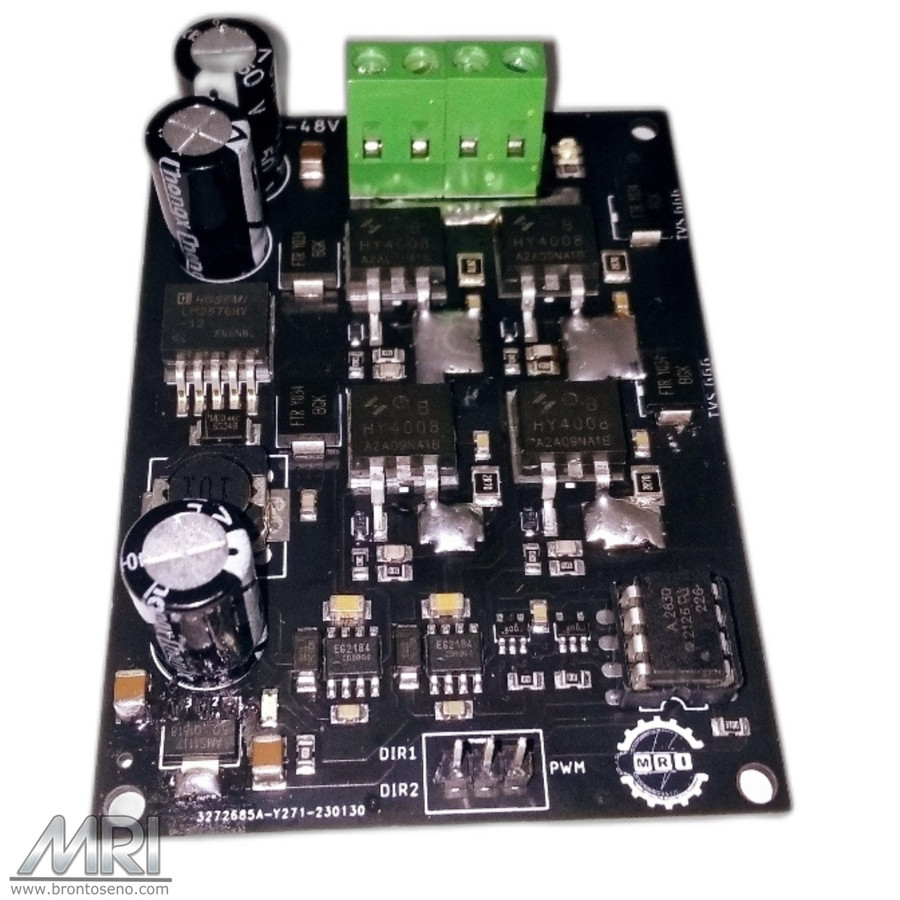
\includegraphics[scale=0.2]{gambar/MotorDriver.png}
        % Keterangan gambar yang diinputkan
        \caption{\emph{H-Bridge Motor Driver}}
        % Label referensi dari gambar yang diinputkan
        \label{fig:DriverMotor}
\end{figure}

Penelitian ini menggunakan \emph{Motor Driver H-Bridge} dari MRI. Perangkat ini dapat digunakan untuk mengatur kecepatan dan arah putar motor \emph{brushed} dengan kapasitas maksimal 50 A pada tegangan 48 V. Driver motor ini dilengkapi dengan satu kanal PWM yang dapat digunakan untuk mengatur kecepatan putar motor dengan cara mengubah lebar pulsa yang dikirimkan ke motor. Lebar pulsa PWM dapat diatur menggunakan potensiometer maupun melalui kontrol sinyal eksternal. Perangkat ini juga memiliki kemampuan untuk mengatur arah putar motor melalui kedua pin dir. Dengan mengganti keadaan \emph{input} kontrol maka pengguna dapat mengubah arah putaran motor secara mudah. Gambar \ref{fig:DriverMotor} merupakan perangkat yang digunakan pada penelitian ini.

\subsection{Kursi Roda Elektrik KY-123}

\begin{figure} [ht]
    \centering
        % Nama dari file gambar yang diinputkan
        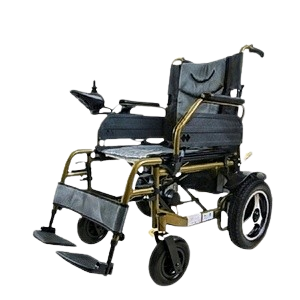
\includegraphics[scale=0.72]{gambar/WheelchairMySellaKY123.png}
        % Keterangan gambar yang diinputkan
        \caption{Kursi Roda Elektrik KY-123}
        % Label referensi dari gambar yang diinputkan
        \label{fig:KY123}
\end{figure}

Kursi roda elektrik sebagian besar terdiri dari rangka kursi roda, alat kontrol gerak kursi roda, motor listrik, serta unit baterai. Alat ini dapat dioperasikan dengan fleksibel, mudah, dan sederhana sehingga tidak memerlukan tenaga yang besar dari pengguna jika dibandingkan dengan kursi roda biasa. Kursi roda ini dapat dioperasikan dengan satu tangan oleh pengguna yang mengalami kelumpuhan hemiplegia. Alat ini juga dapat membantu manula yang susah dalam melakukan mobilisasi. 

Perusahaan MySella telah mengembangkan beberapa model kursi roda elektrik sesuai dengan skenario dan syarat pengaplikasian yang berbeda. Gambar \ref{fig:KY123} merupakan salah satu kursi roda elektrik buatan MySella yang digunakan pada penelitian ini. Kursi roda ini sudah memenuhi persyaratan standar nasional GB 12996-2012. Berikut Tabel \ref{tbl:gb12996} yang menjadi persyaratan standar nasional GB12996-2012.

\begin{longtable}{|l|l|}
    \caption{Standar Nasional GB 12996-2012}
    \label{tbl:gb12996}\\
    \hline
    \multicolumn{1}{|c|}{Parameter} & Indikator Kinerja \\ \hline
    \endfirsthead
    %
    \endhead
    %
    Kecepatan Maksimal              & $\le$ 6 Km/Jam          \\ \hline
    Derajat Kemiringan              & 6\textdegree - 8\textdegree               \\ \hline
    Ketinggian Penghalang           & $\le$ 40 mm             \\ \hline
    Jarak Tempuh                    & $\le$ 20 Km             \\ \hline
    Radius Putar Minimal            & 1.2 m             \\ \hline
    Kemampuan Docking               & 9\textdegree                 \\ \hline
    Lebar Parit                     & 100 mm            \\ \hline
    Suhu Kerja Optimal              & -5\textdegree C - 40\textdegree C           \\ \hline
\end{longtable}

\subsection{Motor DC MY1016Z}

\begin{figure} [ht]
    \centering
        % Nama dari file gambar yang diinputkan
        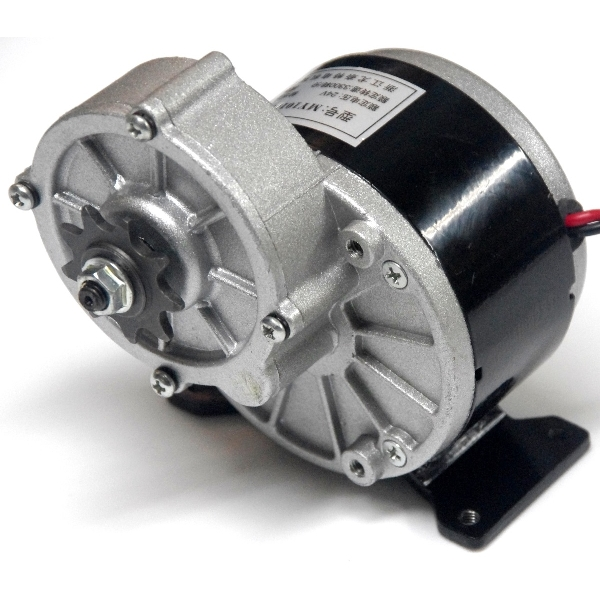
\includegraphics[scale=0.4]{gambar/DCMotorMY1016Z.jpg}
        % Keterangan gambar yang diinputkan
        \caption{Motor DC MY1016Z}
        % Label referensi dari gambar yang diinputkan
        \label{fig:MY1016Z DC Motor}
\end{figure}

Motor DC merupakan jenis dari motor listrik yang menggunakan arus searah untuk menghasilkan gerakan. MY1016Z merupakan \emph{geared} motor DC yang menggunakan mekanisme roda gigi didalamnya. Motor DC ini sering digunakan pada sepeda listrik serta kendaraan sejenisnya. Kursi roda buatan MySella yang bertipe KY-123 juga menggunakan motor DC MY1016Z seperti pada Gambar \ref{fig:MY1016Z DC Motor}.